\documentclass[utf8]{ctexart}

\usepackage[a4paper,left=1.25in,right=1.25in,top=1in,bottom=1in]{geometry}
\usepackage{listings}
\usepackage{graphicx}
\usepackage{caption}
\usepackage{subfigure}
\usepackage{booktabs}
\usepackage{amsmath}
\usepackage{amsthm}
\usepackage{amsfonts}
\usepackage{float}
\usepackage{indentfirst}
\usepackage{tikz}
\usetikzlibrary{shapes,arrows}
\usetikzlibrary{shapes.geometric, arrows}
\usepackage{algorithm}
\usepackage{algorithmic}
\usepackage{newclude}
\usepackage[perpage]{footmisc}

\graphicspath{ {images/} }
%\raggedbottom	% 令页面在垂直方向向顶部对齐
\renewcommand\qedsymbol{QED}
\newcommand{\sign}[1]{\mathrm{sgn}(#1)}
\everymath{\displaystyle}   % 行内公式采用行间公式格式排列
\pagestyle{plain}

\title{《计算机辅助几何设计》第四次作业}
\author{姓名:殷文良\qquad 学号:12435063}
\date{\today}

\begin{document}
\maketitle
\ctexset { section = { format={\Large \bfseries } } }

\section*{思考题 1}
\subsection*{1.}
\begin{itemize}
    \item a.
    \begin{proof}
        由于$C_n^i = C_{n-1}^i + C_{n-1}^{i-1}$,因此
        \begin{equation*}
            M_{i,n}(t) = C_n^it^i
            = (C_{n-1}^i + C_{n-1}^{i-1})t^i
            = M_{i,n-1}(t) + tM_{i-1,n-1}(t).
        \end{equation*}
    \end{proof}
    \item b.
    \begin{algorithm}[H]
        \caption{类 de Casteljau算法}
        \label{alg1}
        \renewcommand{\algorithmicrequire}{\textbf{Input:}}
        \renewcommand{\algorithmicensure}{\textbf{Output:}}
        \begin{algorithmic}[1]
            \REQUIRE $c_i,i=0,1,\dots,n,\quad t\in[0,1]$
            \ENSURE $c_0^n$

            \FOR{$i=0,1,\dots,n$}
            \STATE $c_i^0=c_i$
            \ENDFOR
            \FOR{$k=1,2,\dots,n$}
            \FOR{$i=0,1,\dots,n-k$}
            \STATE $c_i^k = c_{i}^{k-1} + tc_{i+1}^{k-1}$
            \ENDFOR
            \ENDFOR

            \RETURN $c_0^n$
        \end{algorithmic}
    \end{algorithm}
\end{itemize}

\subsection*{2.}
\begin{proof}
    令
    \begin{equation*}
        B_{i,n}'(t) = C_n^i(1-t)^{n-i-1}t^{i-1}(i-nt) = 0,
    \end{equation*}
    可得$t=\frac{i}{n}$,因此$B_{i,n}(t)$在$t=\frac{i}{n}$处达到极值,并且该极值是最大值。
\end{proof}

\subsection*{3.}
\begin{proof}
    设随机变量$\xi$服从二项分布,即
$$
\xi\sim B(n,t).
$$
则其分布列为
$$
P(\xi = i) = B_{i,n}(t),\quad i = 0,1,\dots,n.
$$
于是,$\xi$的期望为
$$
E\xi = \sum_{i=0}^niB_{i,n}(t).
$$
根据二项分布对参数$n$的可加性,以及两点分布$\eta$的期望为$t$,可知
$$
E\xi = nE\eta = nt.
$$
因此,我们有
$$
\sum_{i=0}^niB_{i,n}(t) = nt.
$$
\end{proof}

\section*{思考题 2}
\subsection*{1.}
\begin{proof}
    % 设Bézier 曲线的次数为$n$。\par
    % 若$n=1$,此时Bézier 曲线是一条线段,控制多边形的弦长等于曲线弧长。\par
    % 若$n\geq 2$,由Bézier曲线升阶的收敛性定理可知,控制多边形的弦长收敛于Bézier 曲线的弧长。
    % 由于升阶是一个割角过程,所以控制多边形的弦长不断减小,因此控制多边形的弦长大于曲线弧长。\par
    % 综上,Bézier 曲线的弧长总是小于或等于其控制多边形的边长。
    $$
    \begin{aligned}
        \int_0^1\|P'(t)\|dt &= n\int_0^1\|\sum_{i=0}^{n-1}B_{i,n-1}(t)(P_{i+1}-P_i)\|dt\\
        &\leq n\int_0^1\sum_{i=0}^{n-1}\|B_{i,n-1}(t)(P_{i+1}-P_i)\| dt\\
        &= n\sum_{i=0}^{n-1}\|P_{i+1}-P_i\|\int_0^1B_{i,n-1}(t)dt\\
        &= \sum_{i=0}^{n-1}\|P_{i+1}-P_i\|.
    \end{aligned}
    $$
\end{proof}

\subsection*{2.}
\begin{proof}
    \begin{itemize}
        \item %a 
        由升阶公式可知,$Q_{i} = \frac{i}{n+1}P_{i-1} + (1-\frac{i}{n+1})P_i,i=0,1,\dots,n+1$,其中$P_{-1}=P_{n+1}=0$。于是,$\forall i = 1,\dots,n-1$,
        $$
        \begin{aligned}
        \|Q_{i+1} - Q_i\| &= \|\frac{i+1}{n+1}P_i + (1-\frac{i+1}{n+1})P_{i+1} - \frac{i}{n+1}P_{i-1} - (1-\frac{i}{n+1})P_{i}\|\\
        &= \|\frac{i}{n+1}(P_i-P_{i-1}) + (1-\frac{i+1}{n+1})(P_{i+1}-P_i)\|\\
        &\leq \frac{i}{n+1}\|P_i-P_{i-1}\| + (1-\frac{i+1}{n+1})\|P_{i+1}-P_i\|\\
        &\leq \frac{i}{n+1} s_{\max}(P) + (1-\frac{i+1}{n+1})s_{\max}(P)\\
        &= \frac{n}{n+1} s_{\max}(P).
        \end{aligned}
        $$
        当$i=0$时,
        $$
        \|Q_1-Q_0\| = \|\frac{1}{n+1}P_0  + (1-\frac{1}{n+1})P_1 - P_0\| = \|\frac{n}{n+1}(P_1 - P_0)\| \leq \frac{n}{n+1}s_{\max}(P).
        $$
        类似地,当$i=n$时,$\|Q_{n+1}-Q_n\| \leq \frac{n}{n+1}s_{\max}(P)$.\\
        综上,$s_{\max}(Q)\leq \frac{n}{n+1}s_{\max}(P)$。
        \item %b
        由$a$的结论可知,升阶$r$次后控制多边形最长边
        $$
        s_{\max}(P_r) \leq (\frac{n}{n+1})^r s_{\max}(P) \to 0, \quad r \to \infty.
        $$
    \end{itemize}
\end{proof}

\section*{思考题 3}
\subsection*{1.}
\begin{algorithm}[H]
    \label{alg2}
    \caption{Bézier 曲线交点求解算法}
    \renewcommand{\algorithmicrequire}{\textbf{Input:}}
    \renewcommand{\algorithmicensure}{\textbf{Output:}}
    \begin{algorithmic}[1]
        \REQUIRE $C_1(t),C_2(t)$
        \ENSURE $C_1(t)\cap C_2(t)$
        \STATE $hull1 \gets \text{ComputeConvexHull}(C_1.\text{control\_points})$
            \STATE $hull2 \gets \text{ComputeConvexHull}(C_2.\text{control\_points})$

            \IF{not $\text{ConvexHullsIntersect}(hull1, hull2)$}
                \RETURN []
            \ENDIF

            \IF{$\text{ShouldSplit}(C_1, C_2)$}
                \STATE $(C1\_left, C1\_right) \gets \text{SplitCurve}(C_1)$
                \STATE $(C2\_left, C2\_right) \gets \text{SplitCurve}(C_2)$

                \RETURN $\text{BezierIntersection}(C1\_left, C2\_left)$ \\
                + $\text{BezierIntersection}(C1\_left, C2\_right)$ \\
                + $\text{BezierIntersection}(C1\_right, C2\_left)$ \\
                + $\text{BezierIntersection}(C1\_right, C2\_right)$
            \ENDIF
            \RETURN $\text{ApproximateIntersection}(C_1, C_2)$
    \end{algorithmic}
\end{algorithm}

\subsection*{2.}
\begin{algorithm}[H]
    \label{alg3}
    \caption{$n$次多项式在$[0,1]$上的求根算法}
    \renewcommand{\algorithmicrequire}{\textbf{Input:}}
    \renewcommand{\algorithmicensure}{\textbf{Output:}}
    \begin{algorithmic}[1]
        \REQUIRE $f(x) =\sum_{i=0}^{n}a_ix^i$
        \ENSURE $\{x_i\in [0,1] \vert f(x_i)=0\}$
        \STATE $f(x) =\sum_{i=0}^{n}a_ix^i = \sum_{i=0}^nb_iB_{i,n}(x) = p(x)$
        \RETURN $\text{BezierIntersection}(p(x), y=0|_{x\in [0,1]})$
    \end{algorithmic}
\end{algorithm}

\section*{思考题 4}
\subsection*{1.}
\begin{itemize}
    \item 2维:$p_0 = (-1,0)',
    p_1 = (0,1)',
    p_2 = (2,2)',
    p_3 = (1,0)',
    p_4 = (0,-1)'.$

    \begin{figure}[H]
        \centering
        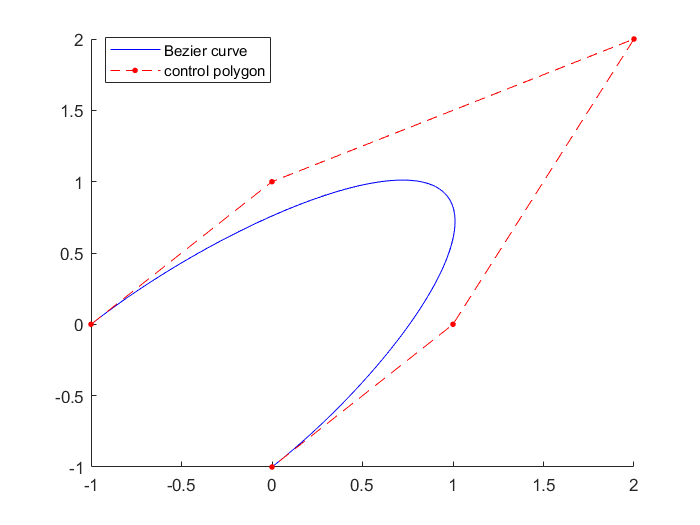
\includegraphics[width=0.8\textwidth]{bezier_2d.png}
        \label{fig1}
        \caption{2维Bézier曲线}
    \end{figure}

    \item 3维:$p_0 = (-1,0,0)',
    p_1 = (0,2,1)',
    p_2 = (2,2,3)',
    p_3 = (1,0,2)',
    p_4 = (0,-1,0)'.$
    \begin{figure}[H]
        \centering
        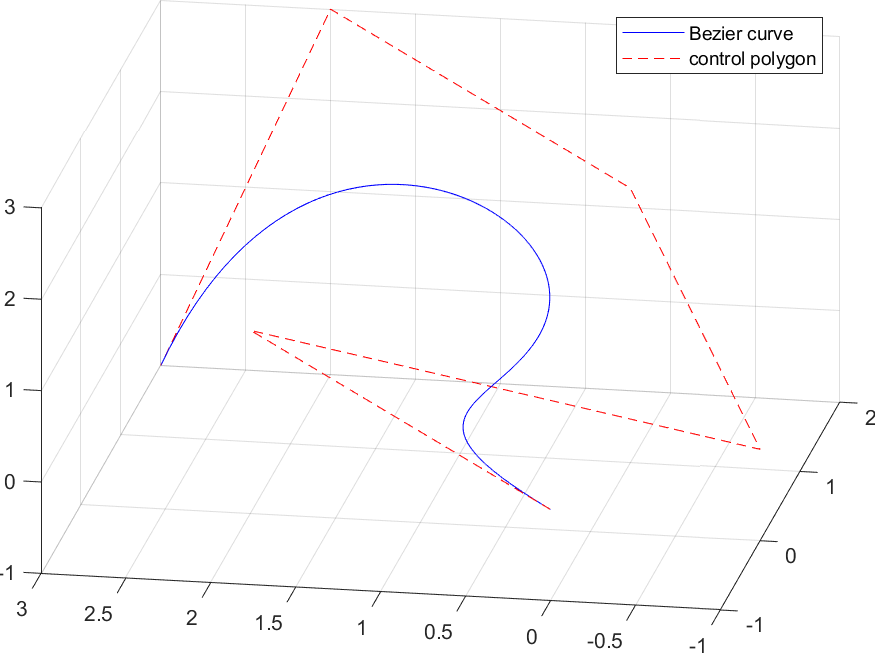
\includegraphics[width=0.8\textwidth]{bezier_3d.png}
        \label{fig2}
        \caption{3维Bézier曲线}
    \end{figure}
\end{itemize}

\subsection*{2.}
\begin{itemize}
    \item 2维:$p_0 = (-1,0)',
    p_1 = (0,1)',
    p_2 = (3,3)',
    p_3 = (1,0)',
    p_4 = (0,-1)'.$

    \begin{figure}[H]
        \centering
        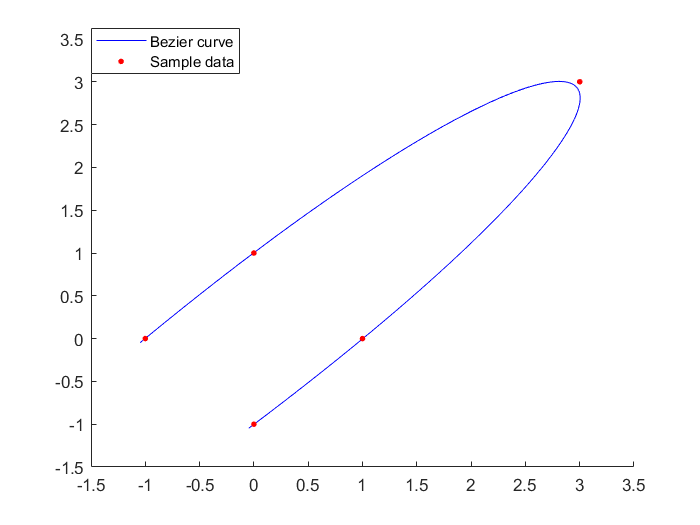
\includegraphics[width=0.8\textwidth]{bezierFit_2d.png}
        \label{fig3}
        \caption{2维Bézier曲线拟合}
    \end{figure}

    \item 3维:$p_0 = (-1,0,0)',
    p_1 = (0,2,1)',
    p_2 = (3,3,3)',
    p_3 = (1,0,2)',
    p_4 = (0,-1,0)'.$
    \begin{figure}[H]
        \centering
        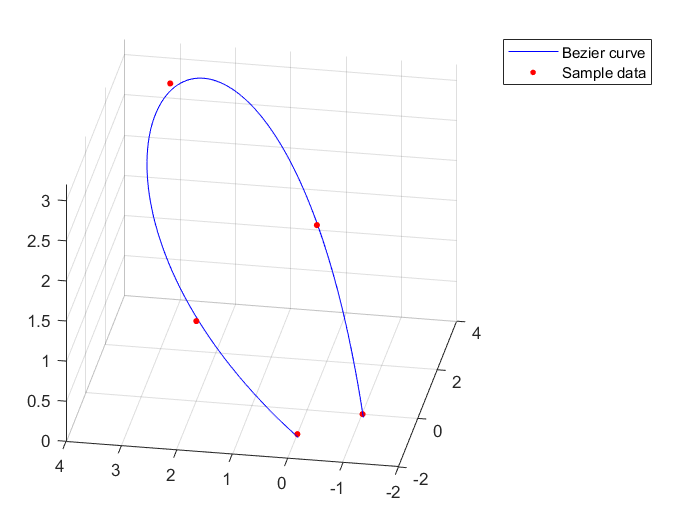
\includegraphics[width=0.8\textwidth]{bezierFit_3d.png}
        \label{fig4}
        \caption{3维Bézier曲线拟合}
    \end{figure}
\end{itemize}

\end{document}
